\chapter{Data Collection and Preprocessing}
\label{chap3}

This chapter describes the data collection process and the preprocessing applied to make the data suitable for the models that will be used later. We will start by explaining how the multiple datasets were acquired, then see how they are joined along with the exploratory data analysis of the final dataset, and finally explore how the ground truths of the task were created.

\section{Overview of Data Sources}

The main datasets used in this thesis are the following 3: the Business Entries Dataset, the Municipal Communities Dataset, and the Neighborhoods Dataset. We will start by seeing how each of these was acquired and what preprocessing modification were made to prepare them for their Exploratory Data Analysis and later practical utilization.


%==================================================
%==================================================
\subsection{Business Entries Dataset}

Our first aim was to collect a dataset of business entries across the city of Volos. In order to do this we collected data from multiple sources and via different methods. Below, we will be breaking down each source and the process of merging them.


% ======================================================
\subsubsection{Foursquare (API Retrieval)}

Foursquare is a global platform that provides information about places and human mobility \cite{foursquare}. In order to acquire data from this source, we used its public API. Specifically, we created a grid of points around Volos \ref{fig:centroids} that represent the centroid of overlapping circles, in order to cover the area of the whole city \ref{fig:centroids_with_area}. 

\begin{figure}[htbp]
    \centering
    \begin{minipage}[b]{0.45\textwidth}
        \centering
        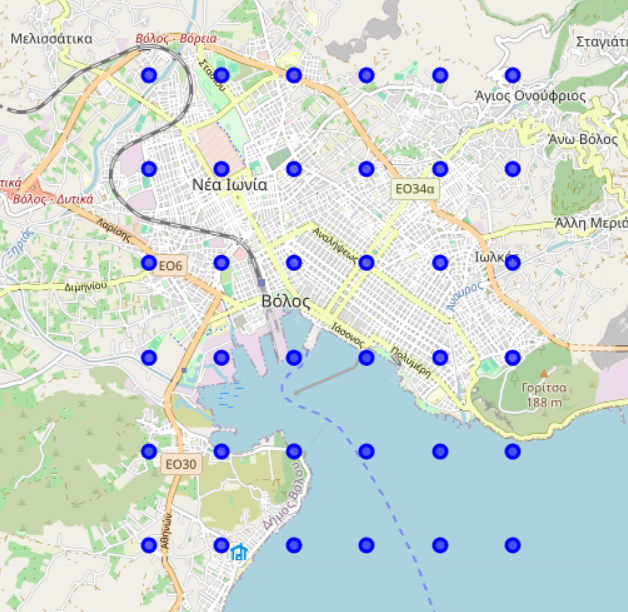
\includegraphics[height=5cm]{figures/centroids.png}
        \caption{Grid Centroids}
        \label{fig:centroids}
    \end{minipage}
    \hfill
    \begin{minipage}[b]{0.45\textwidth}
        \centering
        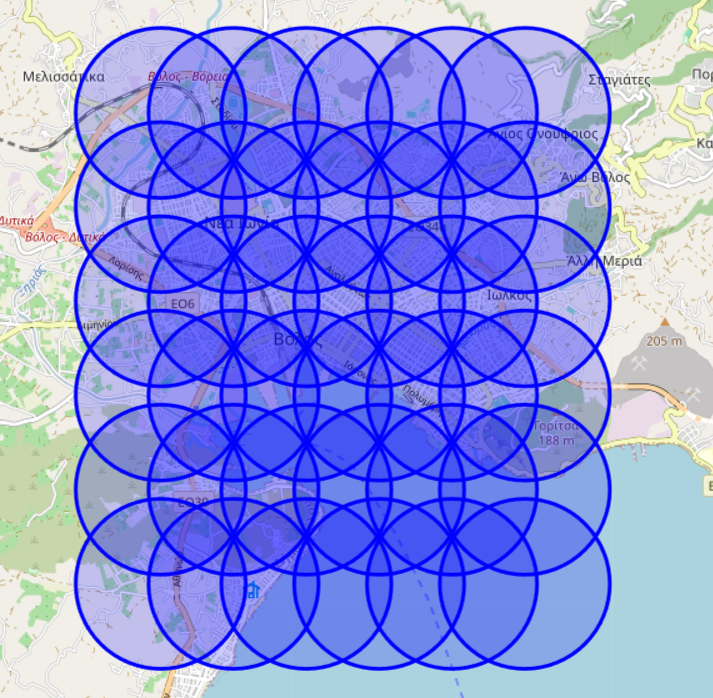
\includegraphics[height=5cm]{figures/centroids_with_area.png}
        \caption{Total Area Covered}
        \label{fig:centroids_with_area}
    \end{minipage}
\end{figure}


An API call was made for each circular area and the results were stored in a JSON file ('places\_\{i\}.json'). Then, we merged the results and deleted the duplicates that occurred due to the area overlapping, and ended up with the final JSON file ('all\_places\_deduplicated.json'). Finally, we transformed the json file into a CSV file in order for the entries to later be able to merge with entries from other sources ('foursquare\_data.csv'). This final file also contains the features 'Rating' and 'Reviews' which we manually added via the Foursquare API for each entry, and also the feature 'Postal Code' that was acquired via the Google Maps API. The total entries of this source were 307. The structure of the Foursquare entries was the following: Name, Address, Rating, City, Postal Code, Latitude, Longitude, Category, Country, Reviews.

%==================================================
\subsubsection{Xrysos Odigos (Web Scraping)}

Xrysos Odigos (Yellow Pages) is a website that contains information about businesses of various categories across Greece \cite{xrysos_odigos}. In order to collect data from this source, the Web Scraper Chrome Extension was used. The raw entries acquired were initially 4364. This source did not provide the 'Latitude' and 'Longitude' features, therefore we performed geocoding through the Google Maps API. The method was successful for 3420/4364 of the entries, so the remaining coordinates were inserted manually, using the Google Maps App. The data was saved in a CSV file ('xrysos-odigos-volos-ratings.csv'). The structure of the Xrysos Odigos entries was the following: Name, Address, Rating, City, Postal Code, Latitude, Longitude, Category, Country, Reviews, Description, Phone.

%==================================================
\subsubsection{Greek Catalog (Web scraping)}

Greek Catalog is an online business directory for Greece, similar to Xrysos Odigos \cite{greek_catalog}. In order to collect data from this source, we utilized the Web Scraper Chrome Extension once more. The raw entries collected were 46 this time. This source did not provide the 'Postal Code' feature, therefore we performed geocoding through the Google Maps API. The data was saved in a CSV file ('greek-catalog-volos.csv'). The structure of the Greek Catalog entries was the following: Name, Address, Rating, City, Postal Code, Latitude, Longitude, Category, Country, Reviews.

%==================================================
\subsubsection{Vacation Renter (Web scraping)}

Vacation Renter is a travel accommodation aggregator that aggregates hotel listings from multiple booking platforms (Booking.com, Vrbo, etc.) \cite{vacation_renter}. In order to collect data from this source, the Web Scraper Chrome Extension was used one final time. The raw entries acquired were 24. This source did not provide the 'Latitude', 'Longitude' and 'Postal Code' features either, therefore the Google Maps API as used to perform geocoding one final time. The 'Category' features was also set to 'Hotel' since this source specifies on this sector. The data was saved in a CSV file ('vacation-renter-volos.csv'). The structure of the data was the following: Name, Address, Rating, City, Postal Code, Latitude, Longitude, Category, Country, Description, Features.

\begin{table}[h!]
    \centering
    \caption{Attribute Presence Across Sources (highlighted were kept)}
    \begin{tabular}{lcccc}
    \toprule
    \textbf{Attribute} & \textbf{Foursquare} & \textbf{Xrysos Odigos} & \textbf{Greek Catalog} & \textbf{Vacation Renter} \\
    \midrule
    \rowcolor{yellow!20}
    Name              & \cmark & \cmark & \cmark & \cmark \\
    \rowcolor{yellow!20}
    Address           & \cmark & \cmark & \cmark & \cmark \\
    \rowcolor{yellow!20}
    Rating            & \cmark & \cmark & \cmark & \cmark \\
    \rowcolor{yellow!20}
    City              & \cmark & \cmark & \cmark & \cmark \\
    \rowcolor{yellow!20}
    Postal Code       & \cmark & \cmark & \cmark & \cmark \\
    \rowcolor{yellow!20}
    Latitude/Longitude& \cmark & \cmark & \cmark & \cmark \\
    \rowcolor{yellow!20}
    Category          & \cmark & \cmark & \cmark & \cmark \\
    \rowcolor{yellow!20}
    Country           & \cmark & \cmark & \cmark & \cmark \\
    \rowcolor{yellow!20}
    Reviews           & \cmark & \cmark & \cmark & -- \\
    \rowcolor{yellow!20}
    Description       & --     & \cmark & --     & \cmark \\
    Phone             & --     & \cmark & --     & -- \\
    Features          & --     & --     & --     & \cmark \\
    Number of Entries & 307    & 4364   & 46     & 24 \\
    \bottomrule
    \end{tabular}
\end{table}

%==================================================
\subsubsection{Merging the Business Data Sources}


On the table below, we can see a review of the structure of the individual data collected from the multiple sources mentioned above, as it has already been modified in order to facilitate their merging. Since the 'Phone' and 'Features' columns only exist in one dataset, we decided to drop them. Regarding the features 'Description' and 'Reviews' which are now the only missing features on some datasets, we simply set their values to Nan in these cases. The actual merging is simple, since all the individual datasets now comprise of the same structure. I ended up with a total of 307 + 4364 + 46 + 24 = 4741 entries, and 11 features.

\begin{figure}[t]
    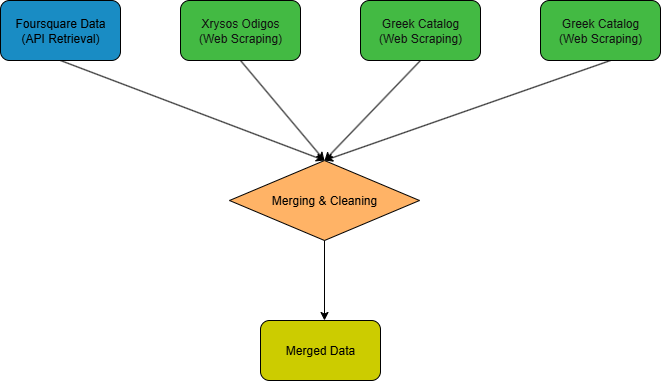
\includegraphics[scale=0.4]{figures/data_merging.png}
    \centering
    \caption{Merging \& Cleaning the Business Data}
    \label{data_merging_cleaning}
\end{figure}

\newpage

%==================================================
\subsubsection{Cleaning the Merged Business Dataset}
Following the concatenation of the individual business datasets, a cleaning process was applied to ensure the final dataset’s integrity and uniformity. Initially, 10 duplicates across the different datasets were identified and deleted. The 'Description' feature, that previously contained unintended line breaks, was reformatted for consistency. A total of 400 entries were found to not actually be located within the administrative boundaries of Volos, and therefore they were eliminated. After verifying the geographical accuracy, some wrongly performed Geocodings were corrected, either manually, or programatically via the Google Maps API, and 1 problematic entry was deleted. 

Multiple entries lacked addresses, so we managed to find and manually insert a proportion, but deleted the 26 remaining. We also excluded 390 records lacking both address and geographic coordinates. Regarding the missing values of the feature 'Postal Code', we manually added them when they were available and removed 3 invalid entries. The feature 'City' also lacked 24 values, which we simply filled with "Βόλος Μαγνησίας". Finally, 4 'Category' values were missing, so we manually inserted them, and deleted 1 invalid record.

Summing up all the records deleted in the cleaning process, we count: 10 + 400 + 1 + 26 + 390 + 3 + 1 = 831, and removing those from the original 4741 we are left with 3910 entries so far.


%==================================================
%==================================================
\subsection{Municipal Communities Dataset}

The next main dataset is the Municipal Communities Dataset. This information was gathered through the ELSTAT platform. This paragraph presents the process of acquiring the raw data and its preprocessing, leading to the creation of the final Municipal Communities Dataset.


%==================================================
\subsubsection{Data Acquisition (ELSTAT)}

ELSTAT is the official national statistics service of Greece \cite{ELSTAT}. It provides detailed demographic, social, and economic data at various administrative levels. Since the final model's recommendations are expected to be areas within Volos, we searched for the smallest geographic unit with available public datasets in ELSTAT. These units were the Municipal Communities, and we kept the ones within the boundaries of Magnesia (76). The platform provided demographic and economic information for each of them.

\begin{figure}[h]
    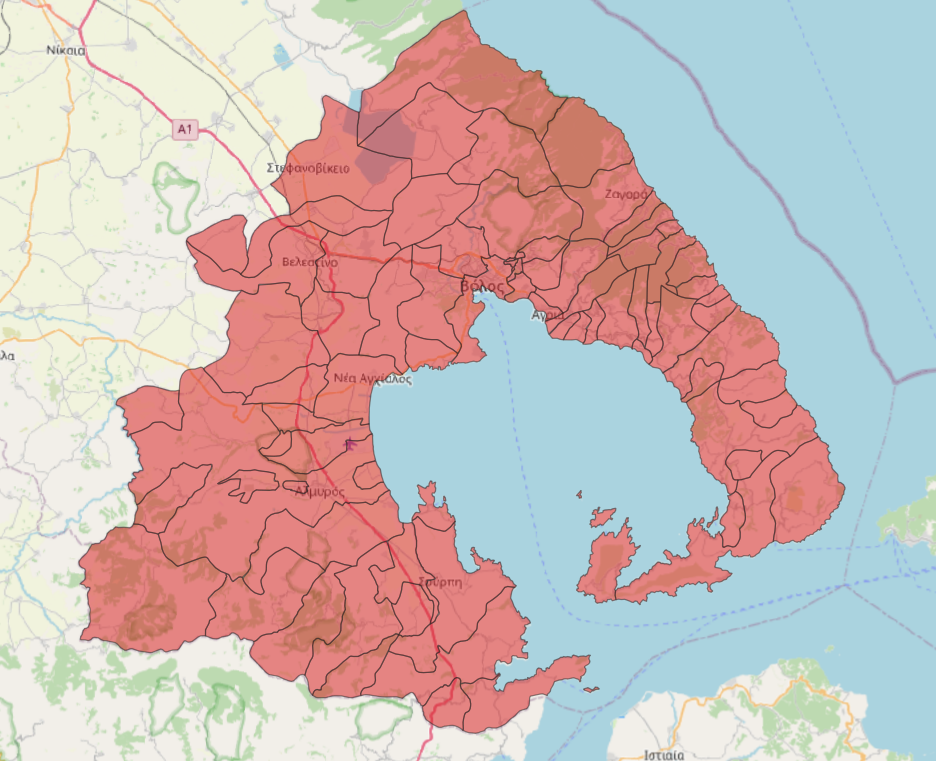
\includegraphics[scale=0.45]{figures/municipal_communities_magnesia.png}
    \centering
    \caption{Municipal Communities within Magnesia}
    \label{municipal_communities_magnesia}
\end{figure}


The demographic data \ref{tab:demographic_columns} contain the population count of each record, along with information about age, educational and marital status groups. More precisely, the age groups are divided to five-year intervals, while the education levels are categorized into six levels. Marital status is recorded as single, married, widowed, or divorced. The total features provided are 32.

The economic features acquired from the ELSTAT platform \ref{tab:economic_columns} are organized hierarchically. The root feature 'Σύνολο' is divided into 'Οικονομικά ενεργοί' and 'Οικονομικά μη ενεργοί'. 'Οικονομικά ενεργοί' is further categorized into 'Άνεργοι' and 'Απασχολούμενοι', while the latter is finally splitted into 'Πρωτογενής', 'Δευτερογενής', 'Τριτογενής'. The total features provided are 12.

The merging of demographic and economic features was simple, since they reference the same municipal community records. The economic and demographic datasets had 4 features in common ('ΠΕΡΙΦΕΡΕΙΑΚΗ ΕΝΟΤΗΤΑ', 'ΔΗΜΟΣ', 'ΔΗΜΟΤΙΚΗ ΕΝΟΤΗΤΑ', 'ΔΗΜΟΤΙΚΗ ΚΟΙΝΟΤΗΤΑ'), so the total number of features ended up being 32 + 12 - 4 = 40. The shape of the dataset is therefore 76x40 so far.


%==================================================
\subsubsection{Feature Engineering}

After merging the demographic and economic datasets, preprocessing steps were applied to guide the feature selection and engineering so the final dataset is enhanced for later analysis. The first transformation applied was to normalize the raw count values for the demographic features of age, education, and marital status groups. This is done to put the features on a comparable scale and to be better fitted for their eventual integration with machine learning models, which benefit from normalized scales.\\

\begin{figure}[H]
    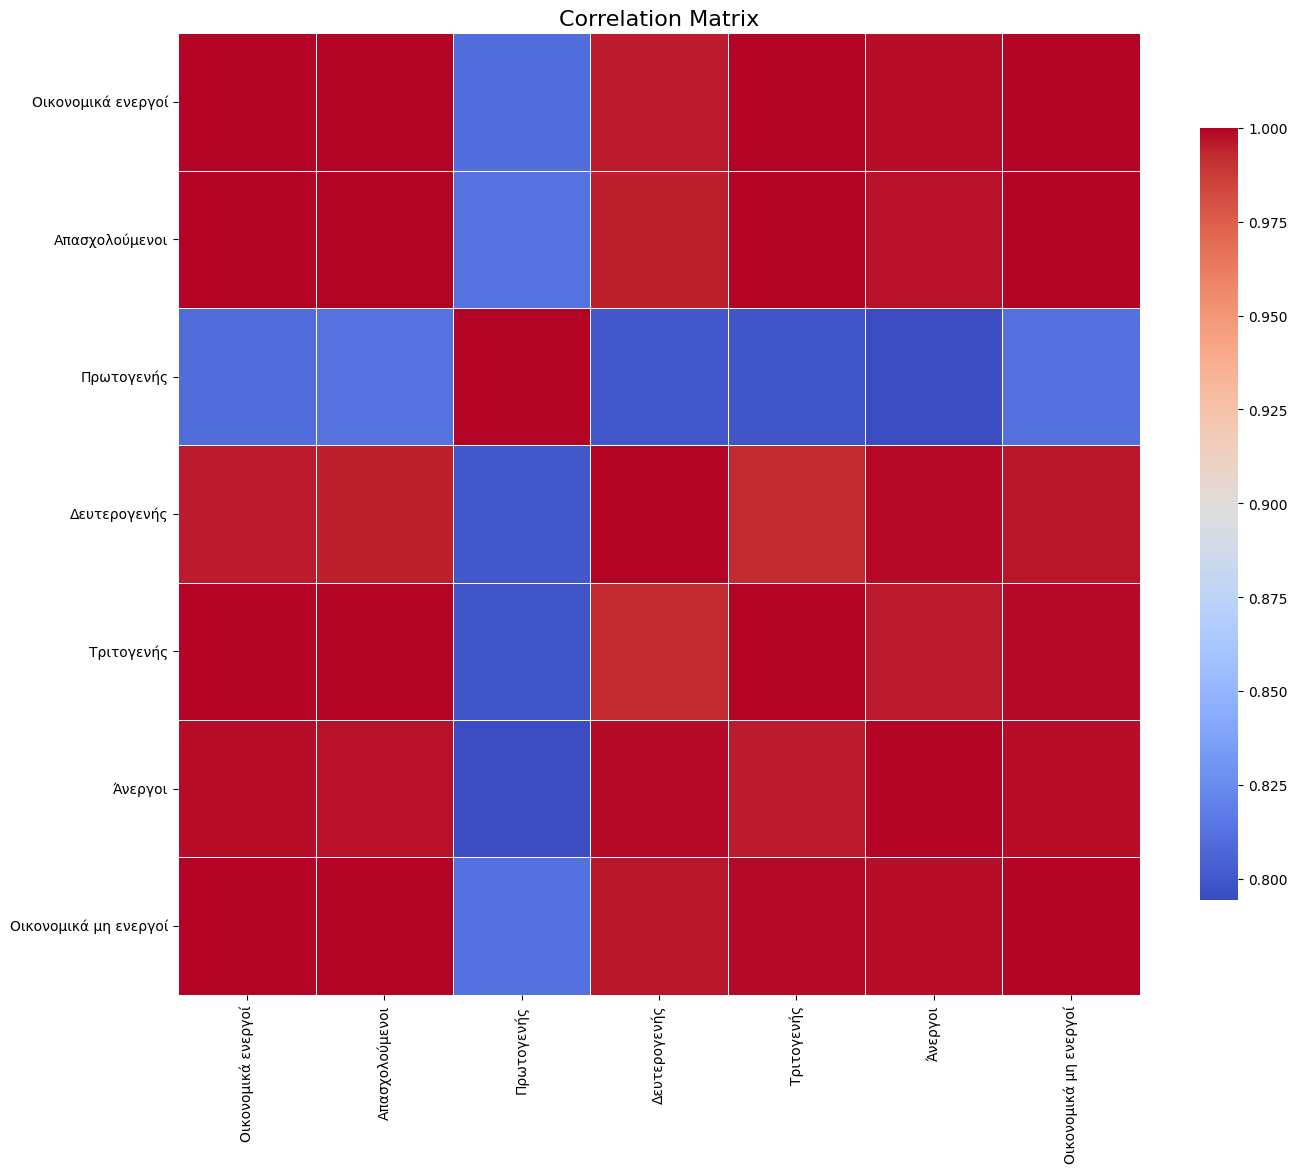
\includegraphics[scale=0.3]{figures/multicoll4.png}
    \centering
    \caption{Correlation Matrix of Economic Features}
    \label{multicollinearity_economic}
\end{figure}

The raw economic features were organized hierarchically, meaning that they contained redundant information. This can be verified by applying a correlation matrix that demonstrates their strong multicollinearity \ref{multicollinearity_economic}. Therefore, we used them to extract some meaningful economic features, like unemployment rate, labor force participation rate, and primary, secondary, and tertiary sector rate. The equations used to extract them from the old features are described in \ref{sec:elstat_feature_engineering}.

In order to reduce the dimensionality of the dataset, we narrowed down the features within age ($15 \rightarrow 3$), educational level ($6 \rightarrow 3$) and economic feature groups ($8 \rightarrow 5$) \ref{sec:elstat_feature_engineering}. The old features were eliminated. The marital status group was not changed. 

In addition, the feature 'Area\_km2' was added through the use of QGIS, which represents the total land area of the municipal community measured in square kilometers. This was possible because, apart from their tabular data, ELSTAT also provided the shapefiles for the geographical units.

I also added a feature with the English name of the Municipal Communities. The final Municipal Communities Dataset has 76 entries and  22 features \ref{tab:final_municipal_communities_columns}.


%==================================================
%==================================================
\subsection{Neighborhoods Dataset}

While the Municipal Community level data are indeed useful, their unit's size is large for the task we aim to achieve. Ideally, we would like smaller geographical units to represent the candidate locations. Therefore, we also created the Neighborhoods Dataset. This paragraph presents the process of acquiring data on the neighborhood level.


%==================================================
\subsubsection{Data Acquisition (QGIS)}

QGIS (Quantum Geographic Information System) is a free and open-source GIS software used for viewing, editing, and analyzing geospatial data \cite{QGIS}. To help acquire spatial data, it provides a QuickOSM plugin, which allows querying and downloading OpenStreetMap data based on specific tags and spatial filters. We used multiple filters (neighborhoods/villages/suburbs/...) to make queries within Volos and therefore received multiple layers, both of point and polygon type. After processing them, we merged them into 1 point layer and stored them as a shapefile ('merged\_neighborhood\_points.shp').

In order for each business entry to be able to be matched to its corresponding neighborhood later, the shapefile should also possess a geomgetry attribute. To achieve this we applied Voronoi Polygons to transform the Point Layer to a Polygon Layer and saved it into another shapefile ('final\_voronoi\_output.gpkg'). The Voronoi Polygons tool partitions space into regions such that every location within a polygon is closer to its generating point (in this case, the neighborhood point layer) than to any other point \cite{Voronoi_polygons}. In \ref{neighborhoods_magnesia} we can see the initial point layer and the produced polygon layer.\\


\begin{figure}[h]
    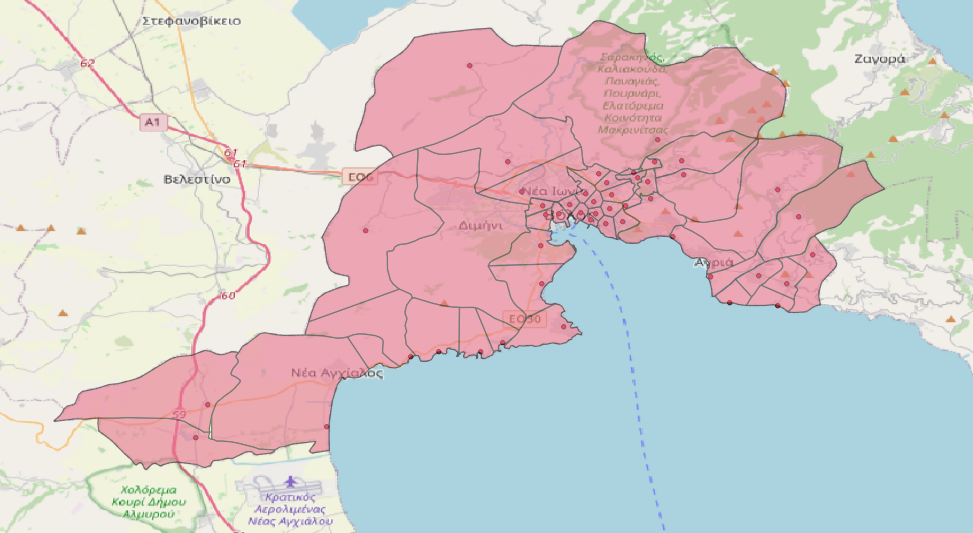
\includegraphics[scale=0.6]{figures/neighborhoods_magnesia.png}
    \centering
    \caption{Neighborhoods within Magnesia}
    \label{neighborhoods_magnesia}
\end{figure}


%==================================================
\subsubsection{Feature Engineering}

Next, we followed a feature enhancement process, that provided some additional features by utilizing QGIS. We were able to extract the centroid coordinates ('x\_centroid', 'y\_centroid') and the polygon area ('area\_km2') for each neighborhood.

We also collected the distance of every neighborhood from various Points Of Interest (POIs). The city center and the port were represented by fixed points, so the distance of each neighborhood to these POIs was measured as the distance between those fixed points and the neighborhood centroids.

Certain POIs, such as main roads, transport stations, and universities, are represented by multiple points or lines. Consequently, I used the QuickOSM plugin to extract a shapefile for these cases. Then, for each neighborhood centroid, the nearest geometry was identified using the 'geopy' library. The final form of the Neighborhood dataset consists of 48 entries with 11 features so far \ref{tab:neighborhood_columns}.


%==================================================
%==================================================
%==================================================
\section{Datasets Integration}


In the previous section, we analyzed how the 3 main datasets were created. In this section, we will see how they are integrated with each other and how the total features end up being greatly enriched in comparison to the initial business dataset. We will start by showing how the NACE code is assigned to each business and then see how we join it with its corresponding municipal community and neighborhood.


%==================================================
\subsection{NACE Code Integration}

In order to standardize business activity classification, the next step was the integration of the NACE code for each business entry. The workflow for this task involved the isolation of all the unique "Category" feature values, and their mapping to their corresponding NACE code. This mapping was performed manually to ensure accuracy, given the variability in category naming across sources. Once it was completed, it was joined with the merged dataset, to add the NACE code and description to each record. In the course of the aforementioned process 4 invalid entries were spotted and deleted, leading to the final number of business records being 3906. 


\begin{figure}[h]
    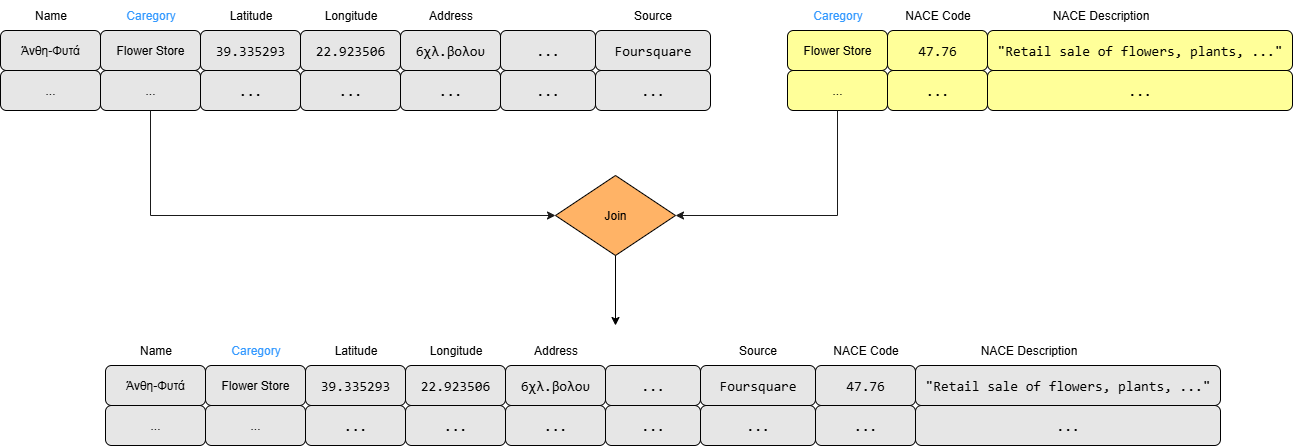
\includegraphics[scale=0.35]{figures/business_nace_join.png}
    \centering
    \caption{Integrating NACE code to the Business Data}
    \label{data_nace_integration}
\end{figure}


Since we added these 2 features, plus we added a 'Source' feature that identifies where I extracted the specific entry from, the shape of the final business dataset is: 3906 entries and 14 columns \ref{tab:business_columns}.


%==================================================
\subsection{Municipal Communities Integration}

Next, we integrated the business entries with the Municipal Communities Dataset. This process consists of two steps: assigning every business to its corresponding municipal community, and merging on this value with the other dataset. The first step was implemented by performing a spatial join between the business dataset and the polygon layer of Municipal Communities programmatically \cite{geopandas_sjoin}. After adding the 'Municipal Community' feature to every entry, we simply join the 2 datasets on it.

\begin{figure}[h]
    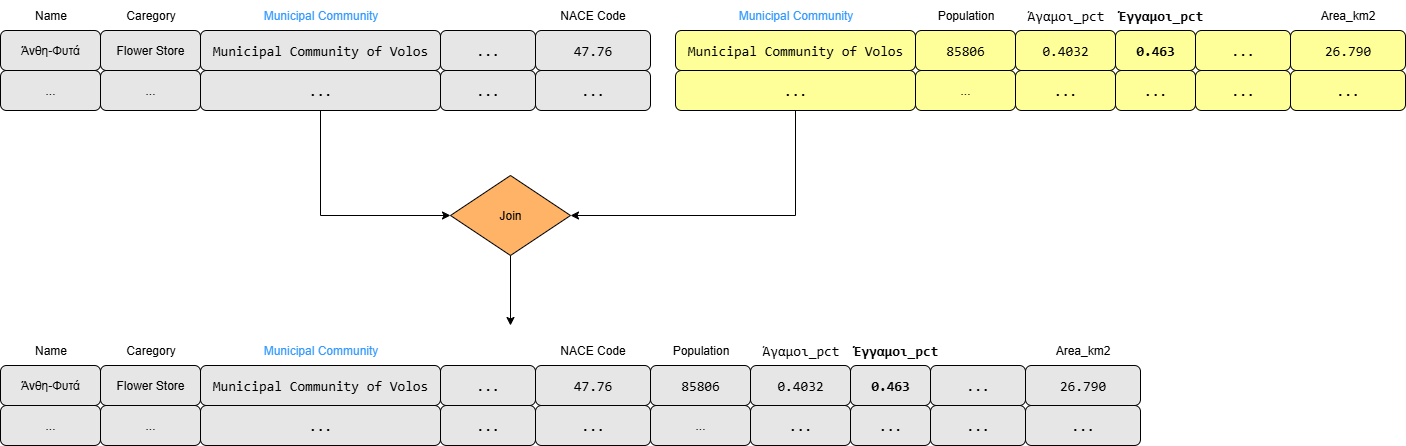
\includegraphics[scale=0.3]{figures/business_mc_join.png}
    \centering
    \caption{Integrating Municipal Community Features to the Business Data}
    \label{data_mc_integration}
\end{figure}

The important part of this process was the 1st step, essentially the enhancement of the business data without necessarily joining the 2 datasets, since this can be done at any time later. The number of entries remains 3906, and the number of features of just the business data is 15 since we just added the 'Municipal Community' feature. If we want to inspect the total features of the joined set, they are 36 since we added the 22 features of the municipal community, and we dropped 'ΔΗΜΟΤΙΚΗ ΚΟΙΝΟΤΗΤΑ ΕΛΛ' as keeping the Greek name was unnecessary.


%==================================================
\subsection{Neighborhoods Integration}

The workflow followed on this paragraph perfectly mirrors the previous one. We perform another spatial join \cite{geopandas_sjoin}, this time assigning each business to its corresponding neighborhood. The spatial join failed for 24 entries because all the neighborhoods belong to the municipality of Volos, while these specific businesses did not, so they were deleted. The valid entries can now be joined to acquire the Neighborhood Dataset features.

\begin{figure}[h]
    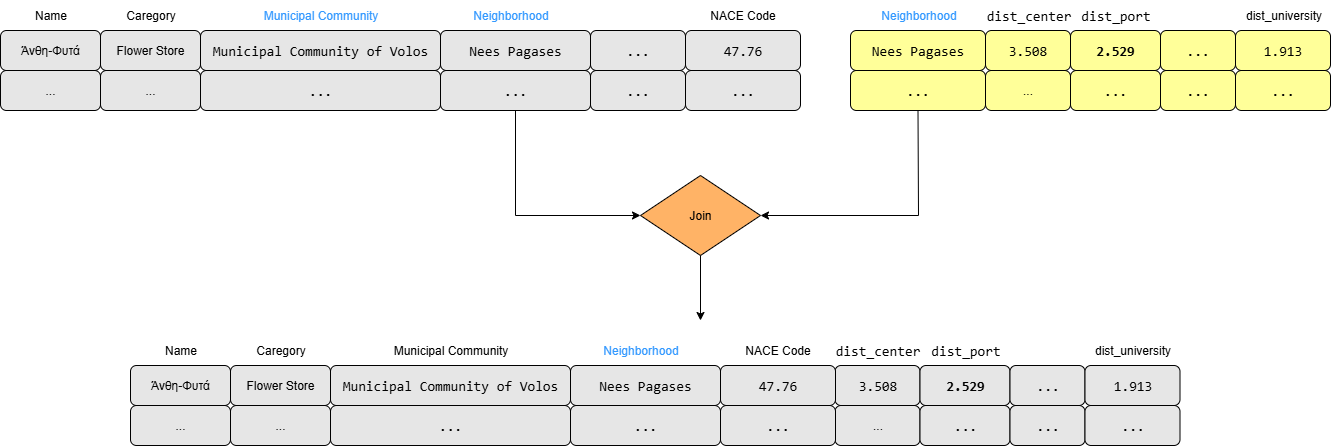
\includegraphics[scale=0.3]{figures/business_neigh_join.png}
    \centering
    \caption{Integrating Neighborhood Features to the Business Data}
    \label{data_neigh_integration}
\end{figure}

As was the case above, the important improvement through this process was the integration of the 'Neighborhood' feature on the business entries. The shape of the business dataset is now 3882 records, due to the 24 invalid spatial joins, and 16 columns since adding 'Neighborhood'. If we look at the fully joined dataset, after joining both on the 'Municipal Community' and 'Neighborhood' features, and keeping only the useful columns for a business entry (dropping 'Geometry', 'Centroid\_x','Centroid\_y', 'Neighborhood\_Greek','ΔΗΜΟΤΙΚΗ ΚΟΙΝΟΤΗΤΑ ΕΛΛ'), their number is 42. In we can see the final schema of the relationships of the 3 main datasets.


%==================================================
\subsection{Integrating Municipal Communities to Neighborhoods}

In the previous two sections we saw how we connect an individual business to its municipal community and neighborhood. However, there is also a connection between the two geographical units themselves, since each neighborhood essentially lies within a municipal community. We can also add the 'Municipal Community' feature to the Neighborhood Dataset by performing a spatial join \cite{geopandas_sjoin} on its centroids with the municipal communities. The added feature results in a 48x12 shape for the neighborhood dataset. After we do this, we can join the neighborhood with the features of its corresponding municipal community. In \ref{data_connection} we can see the final relationship of the 3 main datasets. The arrows act as foreign keys that allow joining on the specific features.


\begin{figure}[h]
    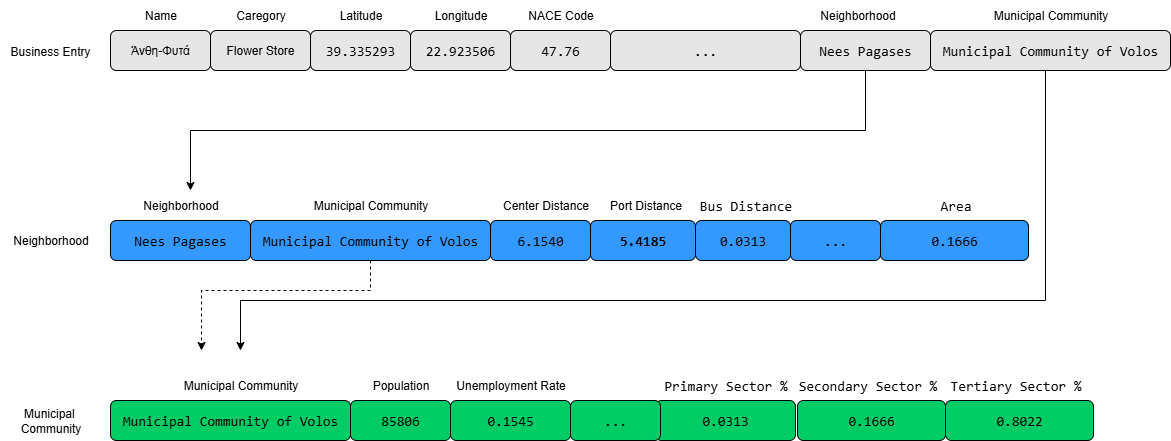
\includegraphics[scale=0.4]{figures/datasets_connected.png}
    \centering
    \caption{Relations of the 3 Datasets}
    \label{data_connection}
\end{figure}


%==================================================
%==================================================
%==================================================
\section{Exploratory Data Analysis}

In the previous sections, we described how we obtained the 3 main datasets and how they are related in order to be joined. In the current paragraph, we will analyze the 3 main datasets individually and then the final joined dataset.


%==================================================
\subsection{EDA - Business Dataset (before joining)}
\label{EDA_business}



We started by inspecting the features of the pure business dataset, before joining it with the other ones. As we mentioned previously, the shape of this dataset is 3882x16. Most of its features are spatial as they provide information about its location. As is obvious, all entries in the 'Country' field are set to 'Greece'. The overwhelming majority of the 'City' column contains the value 'Βόλος Μαγνησίας' (82.86\%), while the next most frequent value is 'Νέα Ιωνία Μαγνησίας' (11.23\%) \ref{fig:city_distr}. The entries contain 12 unique 'Postal Code' values, with '38221', '38333' and '38334' being the most common \ref{fig:postal_distr}. In \ref{business_map_clustered} we can see a clustered version of the businesses on a map, as specifying every point would hinder the clarity of the visualization. We see that most records are located within the city center.

\begin{figure}[h]
    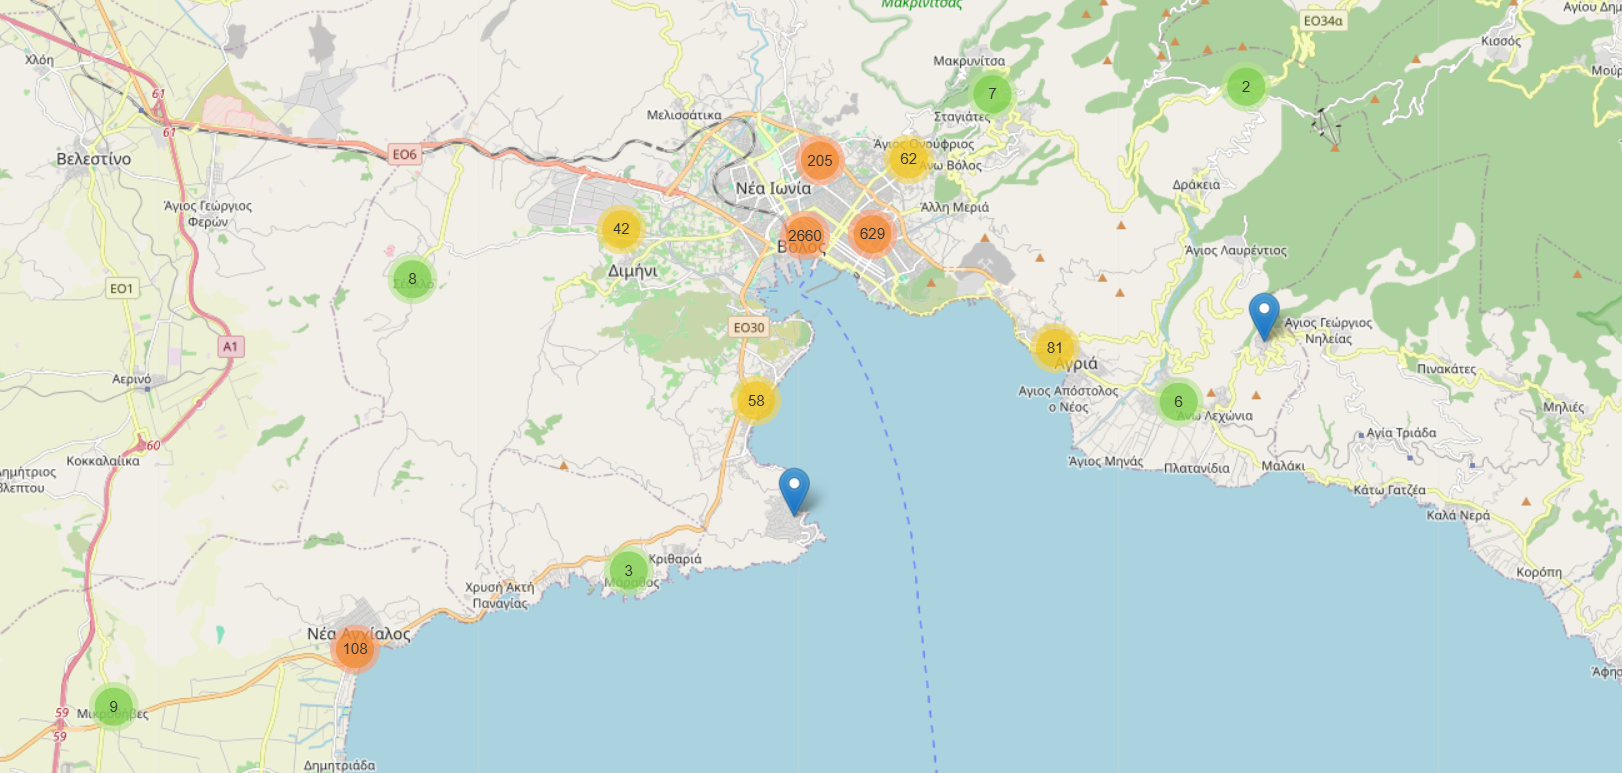
\includegraphics[scale=0.45]{figures/map_clustered.png}
    \centering
    \caption{Clustered Businesses Visualization}
    \label{business_map_clustered}
\end{figure}

\begin{figure}[h]
    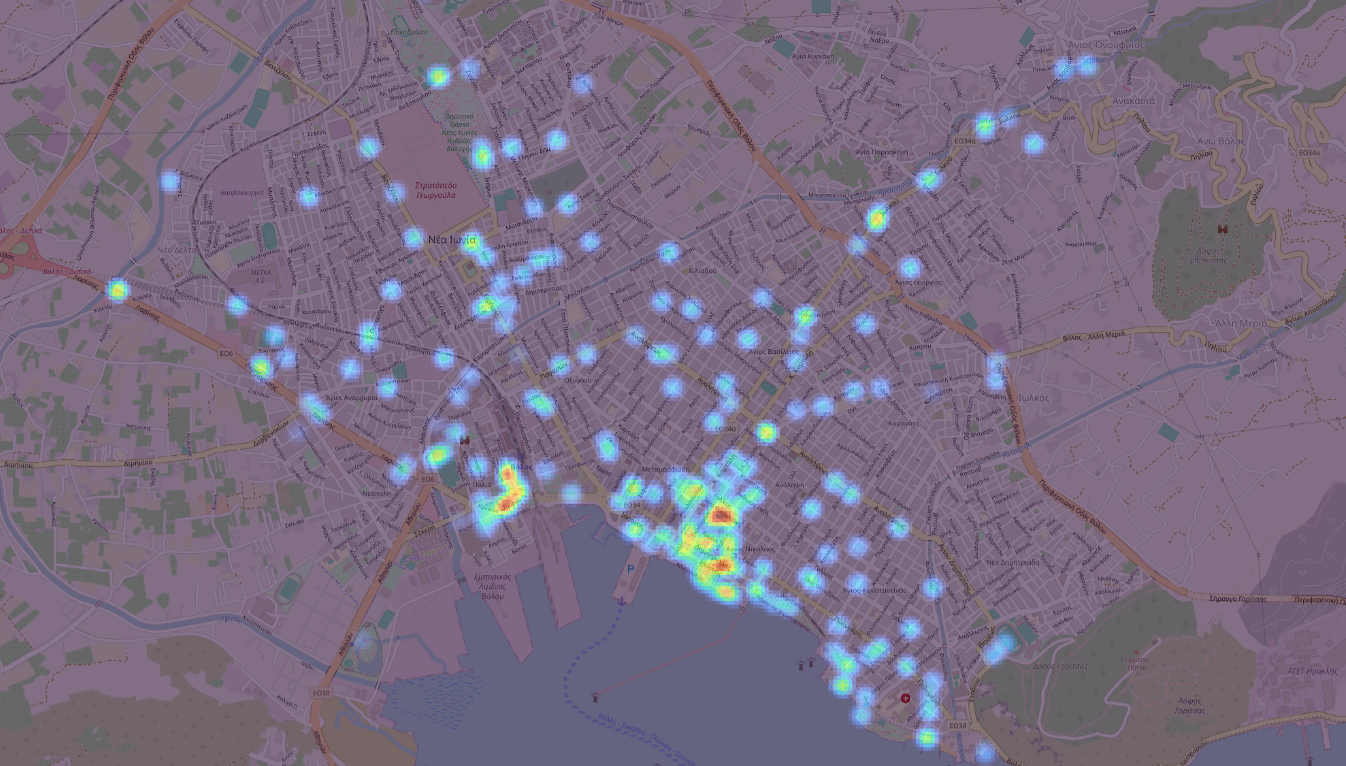
\includegraphics[scale=0.5]{figures/ratings_heatmaps.png}
    \centering
    \caption{'Rating' Feature Heatmap}
    \label{fig:heatmap}
\end{figure}

Although the 'Rating' values are extremely sparse (only 5.87\% present), the distribution of their values is right-skewed \ref{fig:distr_rating}. The figure \ref{fig:heatmap} shows a heat map of the ratings in the city, highlighting their highest values mainly in the center and the Palaia area. Regarding the categorization of the business type, the 'Category' feature consisted of 1233 unique values \ref{fig:category_distr}, while the 'NACE Code' feature only had 306. This is expected since the categogies were the raw values we acquired along with the business entries, while the official categorization method that we will use throughout this thesis is the NACE protocol. In \ref{fig:distr_nace_desc} we can see the most frequent of business types, based on the NACE Code Description. We see that they comprise medical activities, food service and beverage activities, education, and more.

\begin{figure}[h]
    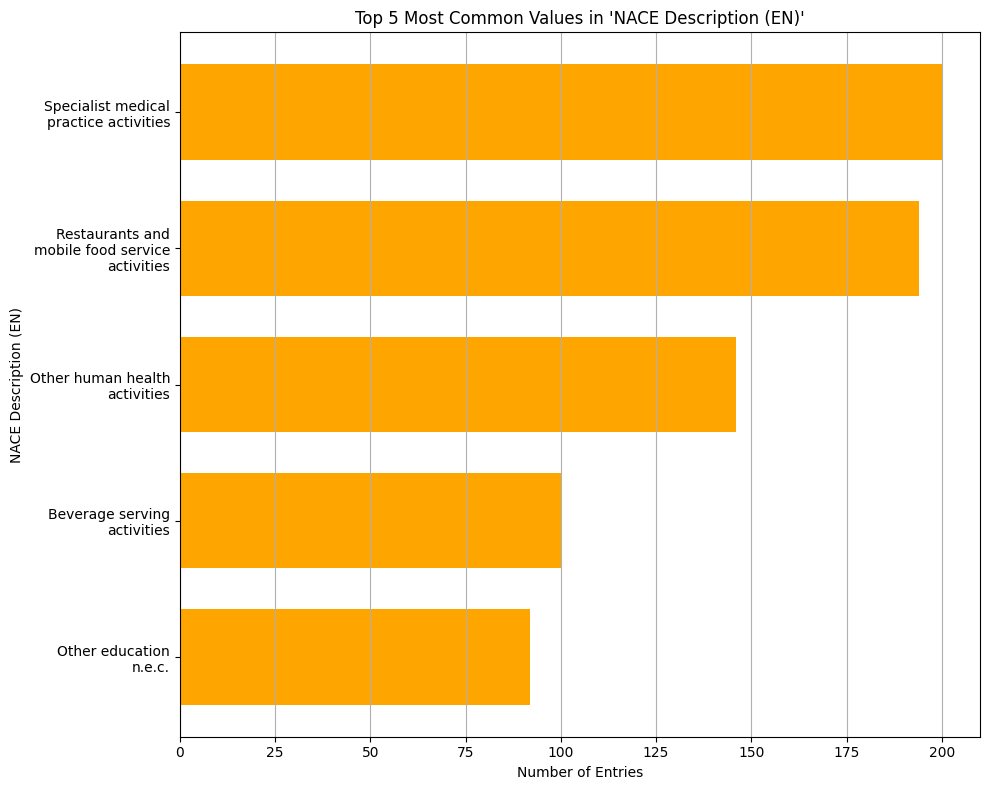
\includegraphics[scale=0.4]{figures/distribution_nace_desc.png}
    \centering
    \caption{'NACE Code' Bar Chart}
    \label{fig:distr_nace_desc}
\end{figure}

Finally, looking into the 'Neighborhood' feature, we can see that its distribution \ref{fig:neighborhood_distr} is much less skewed than the one of 'Municipal Community' \ref{fig:mc_distr}. This is logical because the latter feature refers to a much larger geographical unit which contains the majority of the businesses. The neighborhoods provide a better and informative separation of the areas, and this is why they will be used as the candidates of the recommendation system.  



%==================================================

\subsection{EDA - Municipal Communities Dataset}
\label{EDA_mc}

Subsequently, the Municipal Communities dataset was analyzed, which consists of 76 entries with 23 features. Although 75\% of the spatial units host fewer than 902 people, the municipal communities of Volos and Nea Ionia are outliers, hosting 85.806 and 31.683 respectively. Figure \ref{fig:population_hist} demonstrates the value distribution of the feature, after having removed the 2 extreme outliers mentioned to provide a better visualization. The 'Area\_km2' also contains outliers \ref{fig:box_area}. An attempt was made to identify a correlation between the population and the area features, no sufficient statistical evidence existed to assume such a relationship. The distribution of 'unemployment\_rate' visually suggests a normal distribution approximation. Several statistical tests were applied and did not reject this suspicion while a QQ-Plot strengthened it \ref{fig:stat_unemployment}.

\begin{figure}[h]
    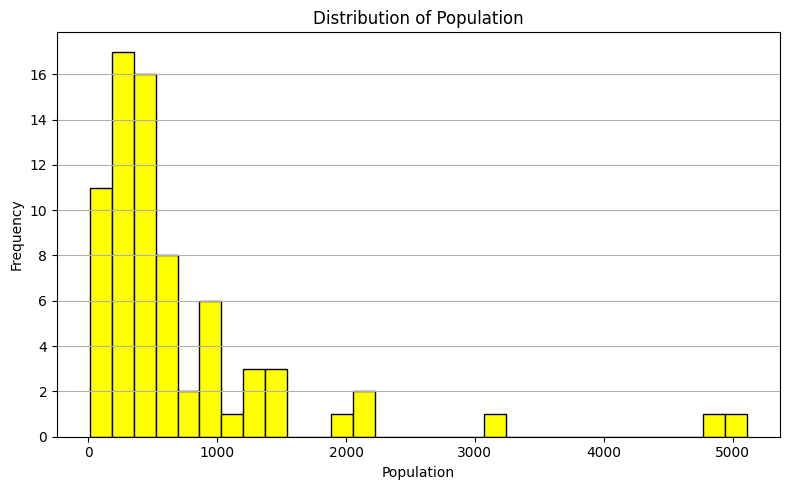
\includegraphics[scale=0.45]{figures/distribution_population_hist2.png}
    \centering
    \caption{'Population' Feature Histogram}
    \label{fig:population_hist}
\end{figure}



The age, education level, marriage and economic sector groups columns comprise feature subsets that suffer internally from multicollinearity since they are perfectly linearly dependent (\ref{fig:corr_age}, \ref{fig:corr_education}, \ref{fig:corr_marriage}, \ref{fig:corr_sector}). Specifically, the percentages of high and low education exhibit a strong negative correlation, as do the percentages of married and unmarried individuals, and the shares of the primary and tertiary sectors. Examining the mean age feature values across all municipal communities shows that the majority of the population is between 10 and 65 years of age \ref{fig:bar_age_mean}. In addition, on average, the majority of the community people posess a low educational level, and higher education levels become progressively less common.
\ref{fig:bar_education_mean}. The mean percentages of married and unmarried citizens correspond to approximately 48.89\% and 35.93\% respectively. Most people are employed in the tertiary sector, followed by the primary and then the secondary sector \ref{fig:bar_sector_mean}.

There is a moderate negative correlation between the 'Population' and the 'age\_65\_plus' columns, which indicates that the most populated municipal communities consist of fewer older people \ref{fig:scat_pop_elderly}. Another relationship I identified was between the unemployment rate and the education level. In particular, it presented a positive correlation with higher education levels \ref{fig:scat_unemployment_high} and a negative correlation with lower education levels \ref{fig:scatter_unemployment_lowed}, both indicating that areas with higher education correspond to lower employment rates. Finally, there is a positive relationship between the proportion of citizens aged 15–64 and labor force participation, which is expected since this age group constitutes the working-age population. \ref{fig:scat_labor_working}.

\begin{figure}[h]
    \centering
    \begin{minipage}[b]{0.45\textwidth}
        \centering
        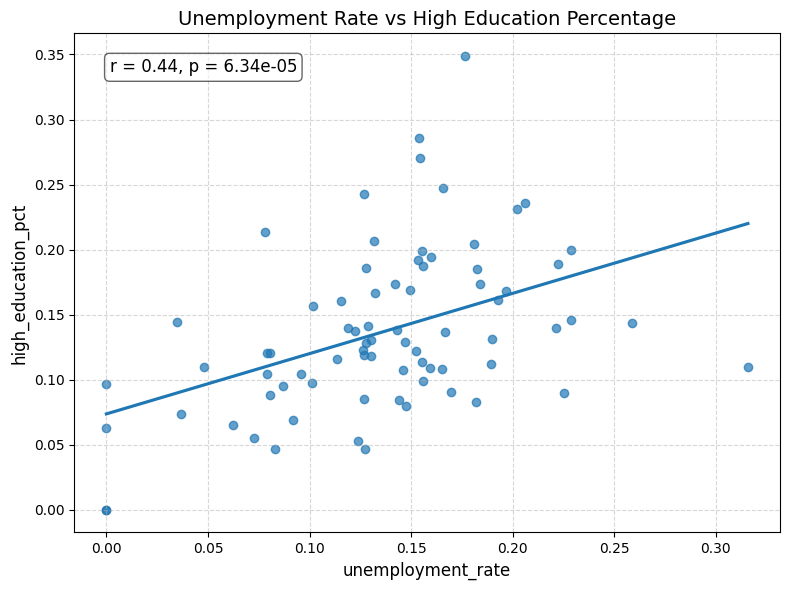
\includegraphics[height=5cm]{figures/scatter_unemployment_highed.png}
        \caption{Scatter Plot: Unemployment Rate VS High Education Level}
        \label{fig:scat_unemployment_high}
    \end{minipage}
    \hfill
    \begin{minipage}[b]{0.45\textwidth}
        \centering
        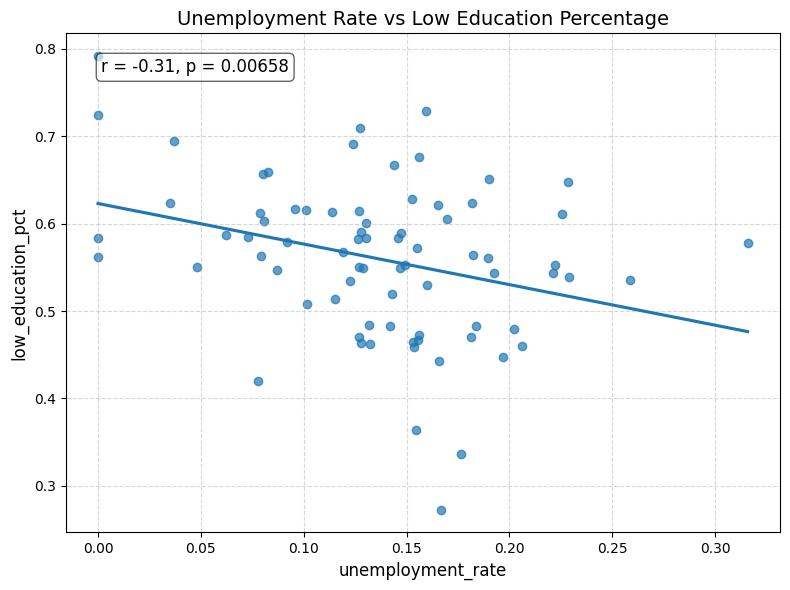
\includegraphics[height=5cm]{figures/scatter_unemployment_lowed.png}
        \caption{Scatter Plot: Unemployment Rate VS Low Education Level}
        \label{fig:scatter_unemployment_lowed}
    \end{minipage}
\end{figure}

%==================================================
\subsection{EDA - Neighborhoods Dataset}


Next, we explored the features of the Neighborhoods Dataset, which consists of 48 entries and 12 total columns. The 'Neighborhood\_Area\_km2' column represents the area of each neighborhood and contains more outliers than the municipal community area \ref{fig:box_area_neigh}. This is caused by the large number of small neighborhoods, particularly those located near the city center, while simultaneously peripheral areas are divided into fewer segments, as we can see in Figure\ref{neighborhoods_magnesia}. The largest areas—Makrinitsa, Glafyra, Dimini, Dimitriada, and Sesklo—also appear as outliers \ref{fig:bar_area_neigh}.

Regarding the distance from the city center, Agios Vasilios, Analipsi, Metamorfosi, Agios Nikolaos and Epta Platania - Oksigono are the most central neighborhoods \ref{fig:bar_center_neigh}. After inspecting the relationship of the neighborhood distance from the city center with various other features, we identified that it presents a positive correlation with many of them. A weak but statistically significant positive relationship with the distance from main roads \ref{fig:scatter_center_highway} confirms the suspicion that central areas tend to have more highways. Its moderate correlation with the distance from transport stops \ref{fig:scatter_center_transport} suggests that public transport is more accessible in central areas. It also presents a nearly perfect correlation with the distance from university \ref{fig:scatter_center_uni}, which shows that, on average, universities are relatively absent from peripheral areas. Another almost perfect linear relationship exist between the distance from the city center and from the city port, which is expected since they are located closely. Finally, a significant direct relationship exists with the neighborhood area \ref{fig:scatter_center_area}, which reflects the shape of the produced Voronoi Polygons and confirms that indeed the peripheral areas are divided into fewer and therefore larger segments. 

\begin{figure}[h]
    \centering
    \begin{minipage}[b]{0.47\textwidth}
        \centering
        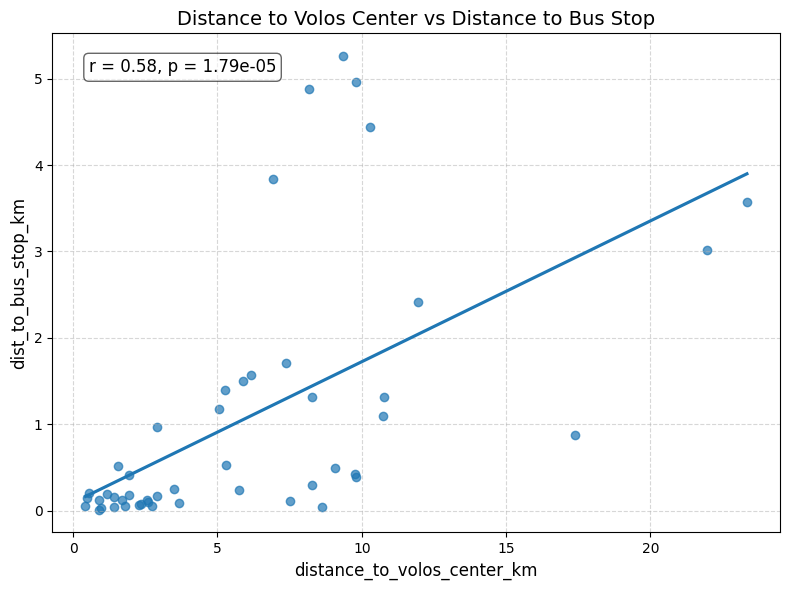
\includegraphics[height=5cm]{figures/scatter_center_transport.png}
        \caption{Scatter Plot: Distance from Center VS Distance from Transport Stops}
        \label{fig:scatter_center_transport}
    \end{minipage}
    \hfill
    \begin{minipage}[b]{0.47\textwidth}
        \centering
        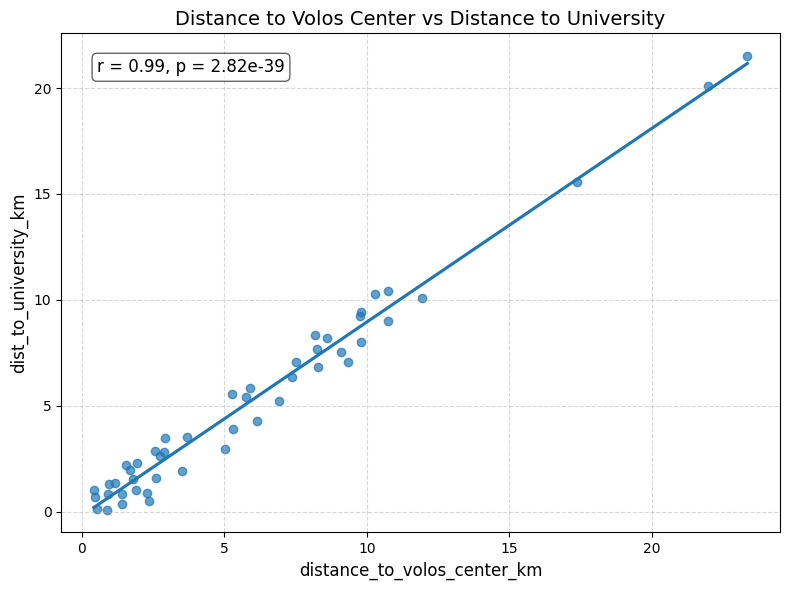
\includegraphics[height=5cm]{figures/scatter_center_uni.png}
        \caption{Scatter Plot: Distance from Center VS Distance from University}
        \label{fig:scatter_center_uni}
    \end{minipage}
\end{figure}

%==================================================
\subsection{EDA - Joined Dataset}

In the three previous sections we inspected and analyzed the 3 main datasets individually. To identify patterns among features originating from different datasets, we present below the analysis of the final joined dataset. It consists of 3882 entries and 42 total features \ref{tab:business_joined_columns}. Inspecting the missing data we see that the dataset is complete, except from the potential label columns ('Rating', 'Reviews', 'Description'), which are very sparse \ref{fig:heatmap_missing}. First, we attempted to relate the business category with several joined features. In order to use fewer categories to get the bigger picture, I grouped the NACE codes by division instead of class and found their mean values across some features. These graphs do not represent a cause and effect relationship between the NACE code and the feature, they just state the context by highlighting observed associations of the columns. 

\begin{figure}[h]
    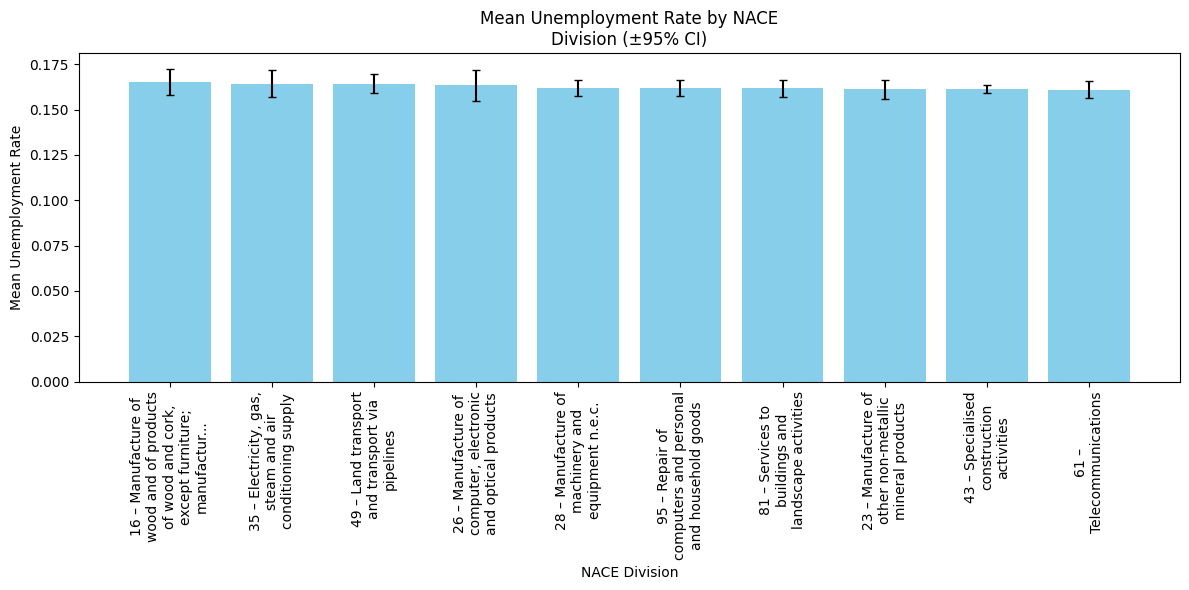
\includegraphics[scale=0.45]{figures/barchart_per_nace_unemployment.png}
    \centering
    \caption{Mean Unemployment per NACE Division Bar Chart}
    \label{fig:barchart_per_nace_unemployment}
\end{figure}

\begin{figure}[h]
    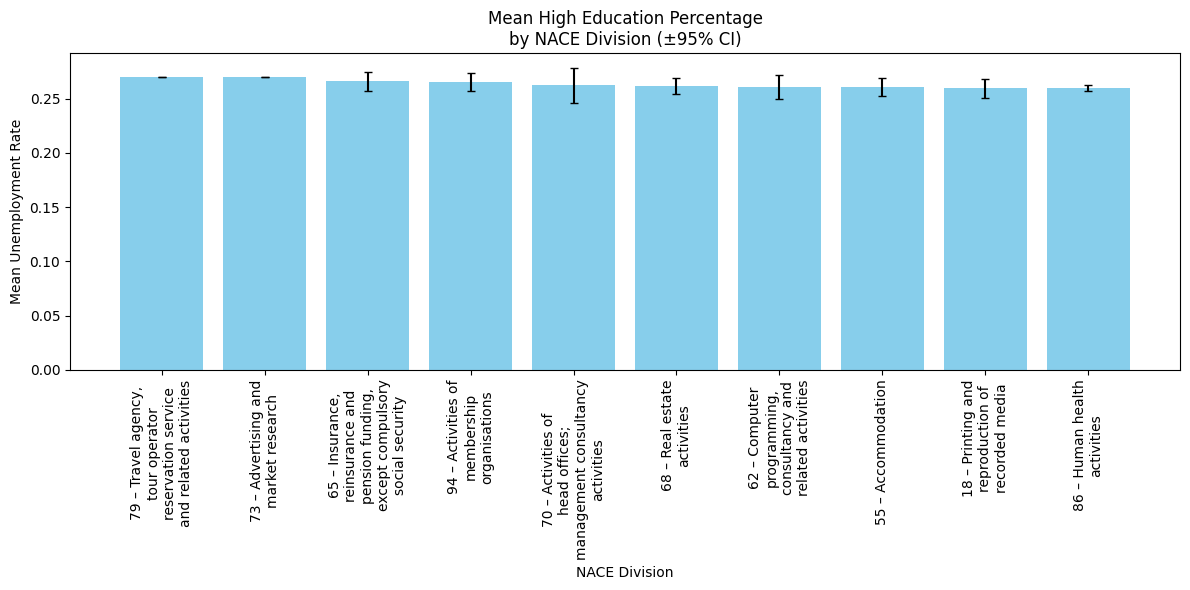
\includegraphics[scale=0.45]{figures/barchart_per_nace_highedu.png}
    \centering
    \caption{Mean High Education per NACE Division Bar Chart}
    \label{fig:barchart_per_nace_highedu}
\end{figure}

Regarding the unemployment rate, although the top values are similar, it is most dominant in the manufacture of wood, electricity and air conditioning supply, land transport, manufacture of computer and electronic products, and manufacture of machinery and equipment \ref{fig:barchart_per_nace_unemployment}. We also see a similar pattern when analyzing the high educational level per NACE division, with the highest values being in the following sections: travel agency, advertising, insurance, activities of membership organisations and management consultancy activities \ref{fig:barchart_per_nace_highedu}.


Despite the severe sparseness of ratings, they present a significant negative relationship with the unemployment rate. To acquire this I calculated the mean rating per municipal community and compared it with the unemployment rate. This indicates that areas that contain highly rated businesses tend to also have a lower unemployment rate value. As before, this only provides context for interpreting rating values that tend to occur alongside specific unemployment rates. I also tried to identify a connection between the rating and the distance from center, but there was no sufficient statistical evidence that supported this suspicion.

\begin{figure}[h]
    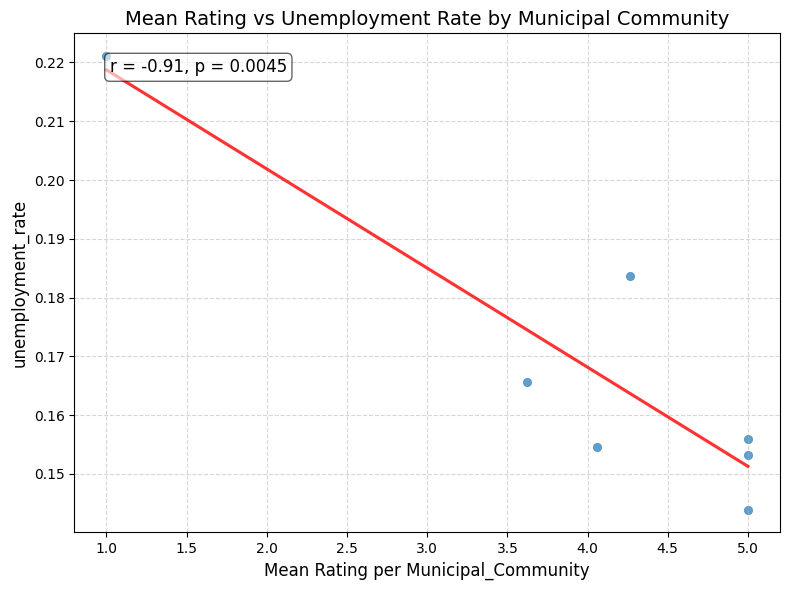
\includegraphics[scale=0.4]{figures/scatter_mean_rating_unemployment.png}
    \centering
    \caption{Scatter Plot: Mean Rating VS Unemployment Rate}
    \label{fig:scatter_mean_rating_unemployment}
\end{figure}




%==================================================
%==================================================
%==================================================
\section{Proxy Ground Truth Creation}
\label{sec:proxy}

In order to utilize machine learning for creating a recommendation system of optimal business locations, we need a criterion to rank the candidate areas for every category to use the top ones as labels. The intuitive approach would be to filter the entries for every NACE class, and use the rating average of every neighborhood to sort the best candidates. This is not feasible, however, due to the sparsity of the labels, so we were forced to create a proxy ground truth myself. 

Following principles of weak supervision and ensemble learning, three complementary approaches were implemented: supervised (learning from labeled instances), unsupervised (capturing latent data structure), and semi-supervised (expanding limited labels). To mitigate the bias of any single method and to also exploit the distinct aspect of the problem space that each approach captures, their outputs were ensembled into a unified ranking. While this does not provide the definitive ground truth, it establishes a consistent and interpretable proxy based on which the models can be trained and evaluated. For every approach, we implemented an attempt that only uses the neighborhood columns, and one that also includes the municipal community features. The two attempts were compared by measuring the amount of central suggestions they provide, and the best was kept.



%==================================================
%==================================================
\subsection{Supervised Learning Approach}

To address the lack of explicit labels, a supervised machine learning approach was first developed. The objective was to approximate the “success likelihood” of each location for a given business category (NACE code).


%==================================================
\subsubsection{Model Dataset Creation}

The worflow begins by creating the dataset that we aim to train the model on. The entries of the dataset consist of every possible (NACE class, Neighborhood) pair, therefore 306x48 = 14688 records. We join the entries with the features of its corresponding neighborhood, and in a second attempt, also with their corresponding municipal communities. The target column does not relate with the ratings, rather it is a new binary value, indicating the presence or absence of a business of this type in a given neighborhood \ref{fig:proxy_approach1}. The dataset presents a considerable class imbalance as only 11.58\% of the label values are 1.

\begin{figure}[h]
    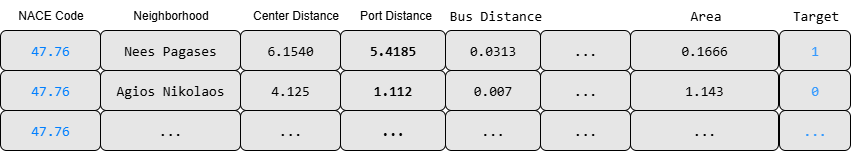
\includegraphics[scale=0.5]{figures/proxy_approach1.png}
    \centering
    \caption{ML Model Dataset Creation}
    \label{fig:proxy_approach1}
\end{figure}


%==================================================
\subsubsection{Top-10 Extraction}

The model used is a Random Forest with 100 decision trees. Prior to training, the input features were scaled to the range [0,1] using 'MinMaxScaler' to ensure comparability with other models in the pipeline. Once trained on the dataset, the model is inferenced to obtain prediction probabilities for every entry. These probability values are then used as ranking criteria for the neighborhoods within each NACE class, with the top 10 being selected as the proxy ground truths. Both attempts resulted in similar lists, but the second was chosen as it yielded a slightly higher percentage of central recommendations (81.48\% over 81.05\%). Although promising, this approach is limited by its implicit assumption that the presence of a business in a location implies a high probability of success, which is not always the case in real world scenarios.



%==================================================
\subsection{Unsupervised Learning Approach}

A second method that uses unsupervised learning was applied, with the goal of identifying the "ideal conditions" for each business category. Unlike the supervised method, this approach does not rely on labels but instead exploits the feature space structure.


%==================================================
\subsubsection{Clustering}

First, we filter the business entries for every NACE class and apply k-means clutering on them. The optimal value of the k parameter is determined by applying the eblow method. After the clusters are created, we determine the "ideal cluster" by comparing them based on the value of a "judge feature", in our case the ratings. Each cluster centroid represents the average profile of the businesses in that group, therefore the centroid of the ideal cluster is assumed to describe the "average ideal conditions" for the specific business type. 

%==================================================
\subsubsection{Top-10 Extraction}

Once the ideal cluster centroid is obtained, we can calculate its Euclidean distance into the same feature space with all the candidate neighborhoods and use it as the ranking criterion. The top 10 recommendations are the 10 neighborhoods closer to the centroid. In \ref{fig:cluster_distance} we see a 2D PCA projection of the high-dimensional feature space containing the candidates and their distance from the ideal cluster centroid for the NACE class 10.52. Although this time the recommendations do not occur solely based on the current business presence, the identification of the “ideal” cluster relies on a single judge feature, oversimplifying the multidimensional nature of business success. 

\begin{figure}[h]
    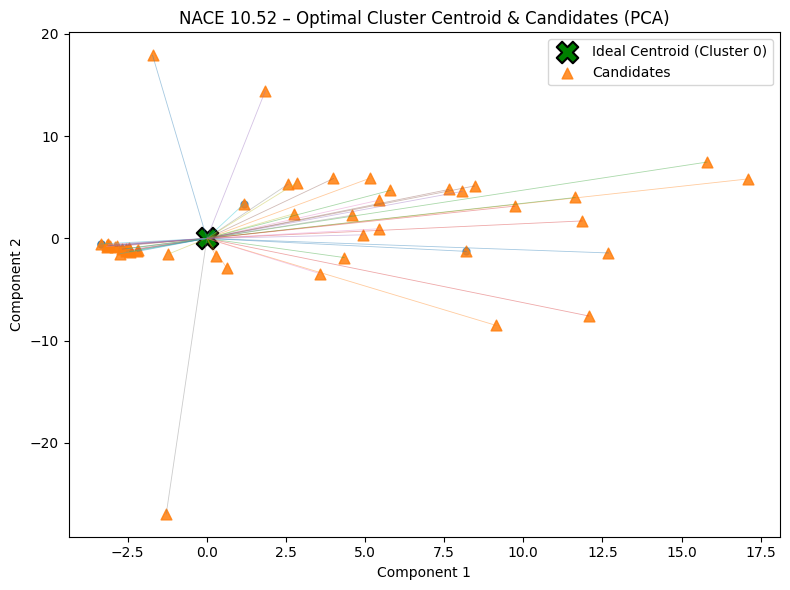
\includegraphics[scale=0.5]{figures/cluster_distance.png}
    \centering
    \caption{Ideal Cluster Centroid \& Candidates (2D PCA)}
    \label{fig:cluster_distance}
\end{figure}



%==================================================
%==================================================
\subsection{Semi-Supervised Learning Approach}

The third method adopted was a semi-supervised learning (SSL) technique, specifically self-training. SSL methods leverage both the limited labeled data and the large pool of unlabeled data by iteratively expanding the training set with pseudo-labels. 

%==================================================
\subsubsection{Self Training}

The model used is a Random Forest Regressor with 100 estimators. The process of self training start with training the initial model on the small set of labeled data (5.87\%). The trained model is then inferenced to produce labels (pseudo-labels) for the unlabeled entries. The pseudo-labels that are predicted "confidently" get integrated to the training set. The model is then re-trained on the updated training set, and the procedure repeats until either all the labels enter the set or no confident predictions occur \ref{fig:psudo_labels}. The confidence of the predictions is determined by comparing its variance to a predetermined threshold explicitly set at 0.1. 


%==================================================
\subsubsection{Top-10 Extraction}

After the ratings are enhanced, we can simply use the mean rating value of each neighborhood as the ranking mechanism to find the optimal locations for each business type. This time only neighborhood features were used since they provided a slightly higher percentage of central locations than the full feature approach. This method resulted to less than 10 recommendations for specific NACE classes since such business types did not exist within every neighborhood, so no rating was created. This is not a problem because the final proxy truths will be determined by combining all three approaches.

\begin{figure}[h]
    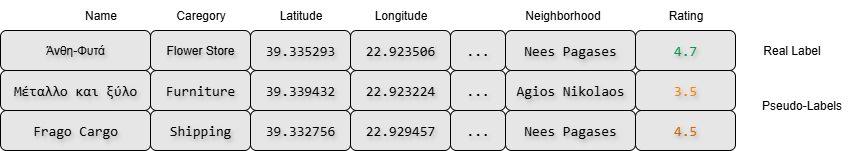
\includegraphics[scale=0.5]{figures/psudo-labels.png}
    \centering
    \caption{Real \& Pseudo Labels}
    \label{fig:psudo_labels}
\end{figure}


%==================================================
%==================================================
\subsection{Ensemble Method}

The techniques outlined in the previous sections capture and contribute an additional view of the problem, but they also suffer from multiple limitations. Following principles of ensemble learning, I combined the individual weaker predictions to obtain the final proxy ground truths. Below, we show a comparison of the individual results and then present their combined outcome.


%==================================================
\subsubsection{Comparison of Results}

Firstly, I compared the three individual proxy truth results to see if they agree or not. I computed the agreement count per NACE class, which essentially combines the total suggestions from all the sources along with their frequency. For example, NACE class 23.70 "cutting, shaping and finishing of stone" presented the following results: 3 votes for Agioi Anargiroi, 3 votes for Nea Ionia, 2 votes for Analipsi, and 1 vote for Epta Platania - Oksigono. In Figure \ref{fig:hist_unique_suggestions} we can see the histogram of the unique suggestions across all NACE classes. A total of 3 suggestions suggest a prefect agreement of the three methods, whereas with more suggestions their results tend to diverge. We see that the majority of different recommendations gathers at 4-6, implying a partial agreement between the techniques.


\begin{figure}[h]
    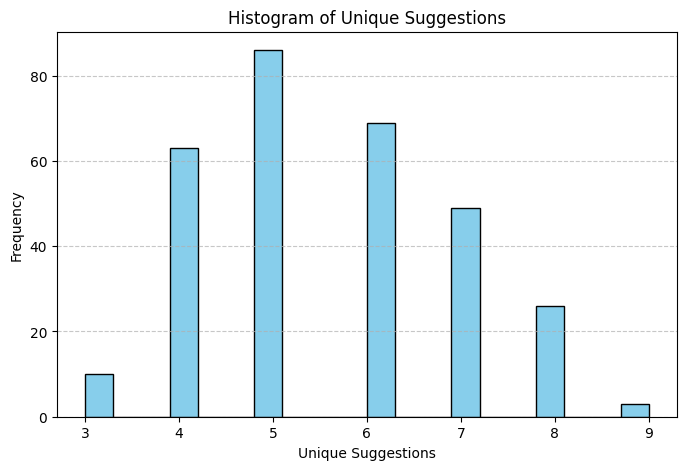
\includegraphics[scale=0.5]{figures/hist_unique_suggestions.png}
    \centering
    \caption{Unique Suggestions of all Methods Histogram}
    \label{fig:hist_unique_suggestions}
\end{figure}


Venn Diagrams can provide a more intuitive understanding of the similarity of the individual suggestions \ref{venn_diagrams}, but they only relate to a specific NACE class and not the wider picture as the histogram did. I also calculated the Jaccard similarity of every NACE class between the pairs of the three aproaches. Figure \ref{fig:barchart_jaccard_similarities} demonstrates the average Jaccard similarity across all NACE classes, and we see that the unsupervised and semi-supervised approach provide the most similar results. Spatial similarity within 1 kilometer was also measured, which measures how geographically close the suggestions are, even when they differ. This also showed that the supervised and unsupervised approaches were the most dissimilars, while the highest similarity was observed between the supervised and semi-supervised approaches.


\begin{figure}[h]
    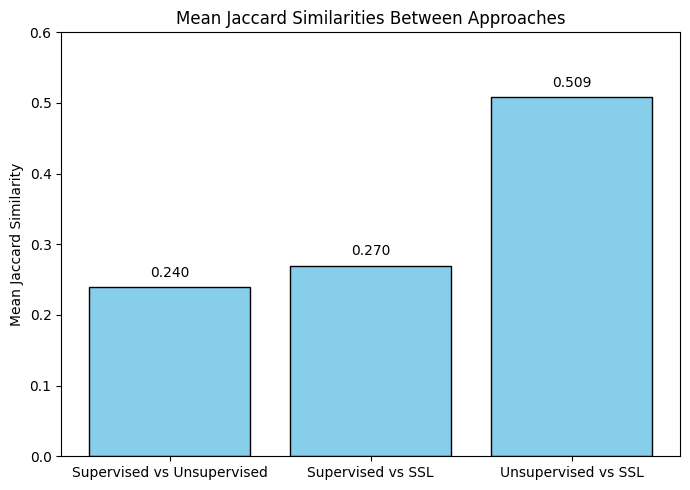
\includegraphics[scale=0.5]{figures/barchart_jacaard_similarities.png}
    \centering
    \caption{Mean Jaccard Similarities Bar Chart}
    \label{fig:barchart_jaccard_similarities}
\end{figure}




%==================================================
\subsubsection{Combination of Results}

To combine the outputs of multiple approaches into a single consensus ranking, a weighted rank aggregation procedure was implemented. Throughout this thesis we have assumed that the central locations tend to be favoured in general, therefore the weight that each approach gets assigned is based on the proportion of its recommendations that fell within the municipality of Volos after being normalized so they add up to 1. In table \ref{tab:weights} we see the central areas pectentage and the corresponding weight of each approach.

\begin{table}[ht!]
    \centering
    \begin{tabular}{|p{5cm}|p{5cm}|p{5cm}|}
        \hline
        \textbf{Approach} & \textbf{Central Suggestions Percentage} & \textbf{Weight} \\
        \hline
        Supervised & 81.48\% & $w_s = 0.3110$ \\ \hline
        Unsupervised & 93.79\% & $w_u = 0.3580$ \\ \hline
        Semi-supervised & 86.67\% & $w_{ss} = 0.3308$ \\ \hline
    \end{tabular}
    \caption{Central Areas Percentage and Weight of Approaches}
    \label{tab:weights}
\end{table}

In addition to method weights, the rank position of each suggested neighborhood was also weighted. Specifically, the following values were assigned: Top1 = 10, Top2 = 9, …, Top10 = 1. This happens to ensure that a candidate appearing higher in a method’s ranking contributed more strongly to the final consensus. In order to obtain the final neighborhood score, we simply perform the weighted sum of the method and rank position \ref{eq:score}: 

\begin{equation}
    \label{eq:score}
    score(N_i) = w_s \cdot top_{s,i} + w_u \cdot top_{u,i} + w_{ss} \cdot top_{ss,i}
\end{equation}

This cumulative score is the final ranking criterion. For every NACE class the candidates were sorted by their scores in descending order and the 10 highest were selected as the final proxy ground truth. In Table \ref{tab:top3} we provide some indicative examples of the final top 3 estimated locations for certain NACE classes.\\

\begin{table}[ht!]
    \centering
    \begin{tabular}{|M{1cm}|M{4cm}|M{3cm}|M{3cm}|M{3cm}|}
        \hline
        \textbf{NACE Class} & \textbf{NACE Description} & \textbf{Top 1} & \textbf{Top 2} & \textbf{Top 3} \\
        \hline
        1.13 & Growing of vegetables and melons, roots and tubers & Metamorfosi & Kato Lehonia & Palaia \\ \hline
        43.22 & Plumbing, heat and air conditioning installation & Agia Paraskeui & Nea Ionia & Agios Georgios \\ \hline
        68.32 & Management of real estate on a fee or contract basis & Agios Nikolaos & Agios Vasilios & Agios Konstantinos \\ \hline
        79.11 & Travel agency activities & Metamorfosi & Agios Konstantinos & Analipsi \\ \hline     
    \end{tabular}
    \caption{Final Top-3 Recommendations of NACE Classes}
    \label{tab:top3}
\end{table}



